\documentclass[12pt,compress,ngerman,utf8,t]{beamer}
\usepackage[ngerman]{babel}
\usepackage{calc}
\usepackage{ragged2e,wasysym,multicol,mathtools,tikz,txfonts}
\usepackage[all]{xy}
\usetikzlibrary{calc,shapes.callouts,shapes.arrows}
\usepackage[protrusion=true,expansion=true]{microtype}
\hypersetup{colorlinks=true}

\graphicspath{{images/}}

\title[Faith in mathematics]{$\varheartsuit$ Faith in mathematics $\varheartsuit$}
\author[Ingo Blechschmidt]{\scriptsize\textcolor{white}{
\vspace*{-1em} \\
\textbf{34th Chaos Communication Congress} \\
\emph{Questions are very much welcome! Please interrupt me mid-sentence.} \\
\medskip
Ingo Blechschmidt (University of Augsburg) \\
with thanks to Matthias Hutzler and Christian Ittner}}

%\usetheme{Warsaw}
\useinnertheme[shadow=false]{rounded}
\useoutertheme{split}
\usecolortheme{orchid}
\usecolortheme{whale}
\setbeamerfont{block title}{size={}}

\useinnertheme{rectangles}

\usecolortheme{seahorse}
\definecolor{mypurple}{RGB}{150,0,255}
\setbeamercolor{structure}{fg=mypurple}
\definecolor{myred}{RGB}{150,0,0}
\definecolor{darkred}{RGB}{240,0,0}
\setbeamercolor*{title}{bg=myred,fg=white}
\setbeamercolor*{titlelike}{bg=myred,fg=white}

\usefonttheme{serif}
\usepackage[T1]{fontenc}
\usepackage{libertine}

\renewcommand{\_}{\mathpunct{.}\,}
\newcommand{\BB}{\mathbb{B}}
\newcommand{\M}{\mathcal{M}}
\newcommand{\R}{\mathrm{R}}
\newcommand{\NN}{\mathbb{N}}
\newcommand{\RR}{\mathbb{R}}
\newcommand{\Eff}{\mathrm{Eff}}
\newcommand{\TM}{\mathrm{TM}}
\newcommand{\STM}{\mathrm{STM}}
\newcommand{\RW}{\mathrm{RW}}
\newcommand{\lambdaC}{\lambda\mathrm{C}}
\newcommand{\PA}{\mathrm{PA}}
\newcommand{\goedel}[1]{\ulcorner #1 \urcorner}
\newcommand{\Prov}{\mathrm{Prov}}
\newcommand{\True}{\mathrm{True}}
\newcommand{\Con}{\mathrm{Con}}
\newcommand{\proves}{\vdash}
\newcommand{\defeq}{\vcentcolon=}

\newcommand{\pointthis}[4]{%
  \tikz[remember picture,baseline]{\node[anchor=base,inner sep=0,outer sep=0]%
    (#3) {#3};\node[overlay,rectangle callout,%
      callout relative pointer={(#1)},fill=blue!20] at
        ($(#3.north)+(#2)$) {#4};}}

\newcommand{\kasten}[1]{%
  \setlength{\fboxrule}{2pt}%
  \setlength{\fboxsep}{8pt}%
  {\usebeamercolor[fg]{item}\fbox{\usebeamercolor[fg]{normal text}\parbox{0.2cm}{#1}}}}%

\newcommand{\slogan}[1]{%
  \begin{center}%
    \setlength{\fboxrule}{2pt}%
    \setlength{\fboxsep}{8pt}%
    {\usebeamercolor[fg]{item}\fbox{\usebeamercolor[fg]{normal text}\parbox{0.88\textwidth}{#1}}}%
  \end{center}%
}

\newcommand{\code}[1]{%
  \begin{center}%
    \setlength{\fboxrule}{1pt}%
    \setlength{\fboxsep}{8pt}%
    {\fbox{\parbox{0.81\textwidth}{#1}}}%
  \end{center}%
}

\setbeamertemplate{navigation symbols}{}

\setbeamertemplate{title page}[default][colsep=-1bp,rounded=false,shadow=false]
\setbeamertemplate{frametitle}[default][colsep=-2bp,rounded=false,shadow=false,center]

\newcommand{\hil}[1]{{\usebeamercolor[fg]{item}{\textbf{#1}}}}
\newcommand{\bad}[1]{\textbf{\textcolor{darkred}{#1}}}
\setbeamertemplate{frametitle}{%
  \vskip1em%
  \leavevmode%
  \begin{beamercolorbox}[dp=1ex,center]{}%
      \usebeamercolor[fg]{item}{\textbf{\textsf{\Large \insertframetitle}}}
  \end{beamercolorbox}%
}

\setbeamertemplate{footline}{%
  \leavevmode%
  \hfill%
  \begin{beamercolorbox}[ht=2.25ex,dp=1ex,right]{}%
    \usebeamerfont{date in head/foot}
    \insertframenumber\,/\,\inserttotalframenumber\hspace*{1ex}
  \end{beamercolorbox}%
  \vskip0pt%
}

\newcommand{\backupstart}{
  \newcounter{framenumberpreappendix}
  \setcounter{framenumberpreappendix}{\value{framenumber}}
}
\newcommand{\backupend}{
  \addtocounter{framenumberpreappendix}{-\value{framenumber}}
  \addtocounter{framenumber}{\value{framenumberpreappendix}}
}

\newcommand{\portrait}[4]{\begin{column}{#3\textwidth}\centering\includegraphics[height=#4\textheight]{#1}\\{\scriptsize #2\par}\end{column}}

\setbeameroption{show notes}

\begin{document}

\addtocounter{framenumber}{-2}

% http://www.ufointernationalproject.com/wp-content/uploads/2015/11/a23.jpg
{\usebackgroundtemplate{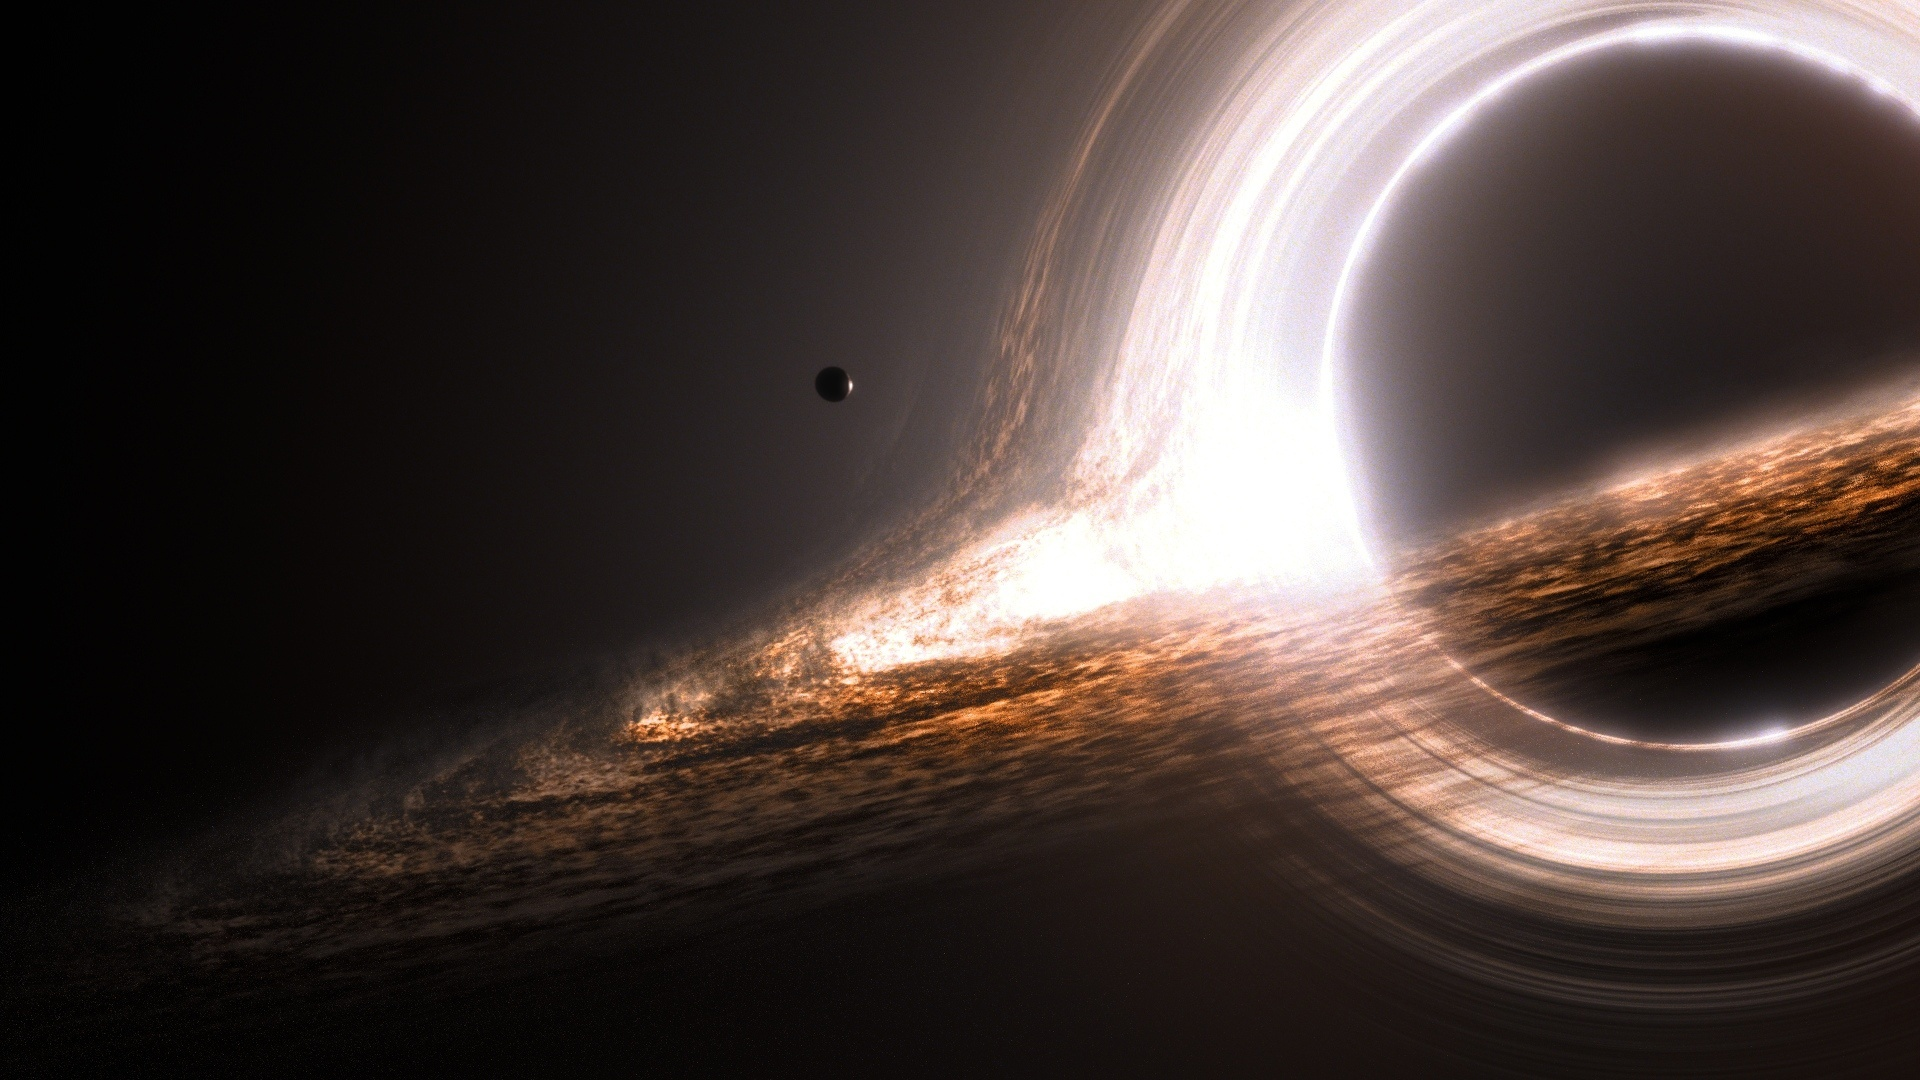
\includegraphics[height=\paperheight]{images/interstellar}}
% https://ecstathy.blogspot.de/2007/10/faith-based-mathematics.html
\frame{\vspace*{1em}
\includegraphics[width=0.4\textwidth]{faith-based-mathematics}\vspace*{2em}\titlepage}}
\frame{\tableofcontents}


\section[Genesis]{Genesis of mathematical logic}

\begin{frame}
  \centering
  \only<1,3-6>{
    \bigskip

    \Huge \textbf{Part I}

    \bigskip
    \Large\hil{The foundational crisis in mathematics}
    \par
    \bigskip
    \bigskip
  }

  \normalsize

  \only<1,3-5>{
    
\includegraphics[width=0.4\textwidth]{principia-mathematica} \\
    \only<3->{
      \mbox{\!\!\!\!``Let $U$ be the set of all those sets which don't contain themselves.''}
    }
    \only<4->{
      \mbox{Naive mathematics is \bad{inconsistent}, rendering it \bad{unreliable}. \bad{\frownie}}
    }
    \only<5>{
      Thus the \hil{axiomatic method} was born.
    }
  }

  \only<2>{
    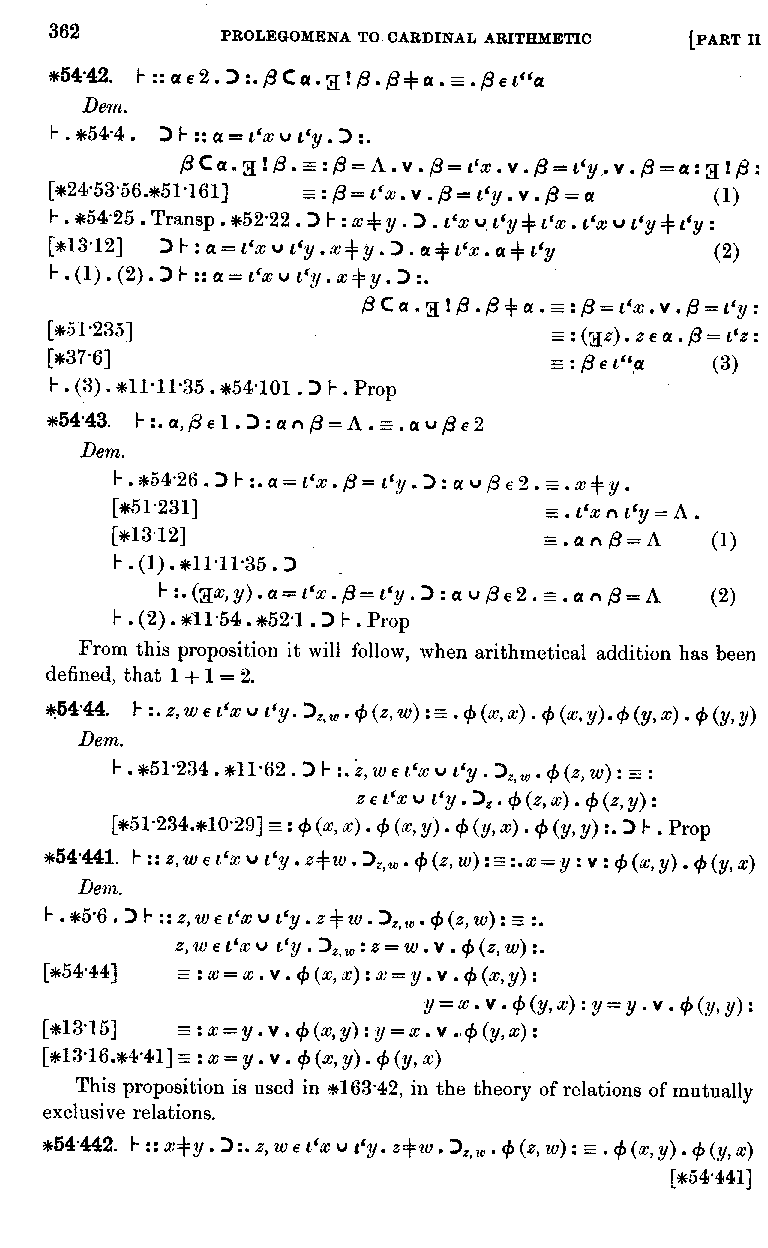
\includegraphics[width=0.5\textwidth]{principia-mathematica-1plus1}
  }

  \only<6>{
    \begin{columns}[t]
      \begin{column}{0.13\textwidth}\end{column}
      \portrait{logicomix}{}{0.37}{0.55}
      \portrait{lovelace-babbage}{}{0.37}{0.55}
      \begin{column}{0.13\textwidth}\end{column}
    \end{columns}
  }
\end{frame}


\section{Truth and proof}

\begin{frame}
  \centering
  \bigskip

  \Huge \textbf{Part II}

  \bigskip
  \Large\hil{Truth and proof}
  \par
  \bigskip
  \raggedright
  \small

  \begin{block}{A syntactic quality}
    A statement is \hil{provable} if and only if it has a \hil{formal proof}
    using only the \only<1>{\hil{Peano
    axioms}}\only<2->{\hil{\pointthis{-0.5cm,-1.7cm}{1.5cm,3.1cm}{Peano
    axioms}{\textnormal{\textcolor{black}{\begin{minipage}{0.7\textwidth}Mathematical
    induction
    and:\begin{align*}
      S(n) &\neq 0 &
      S(n) &= S(m) \Rightarrow n = m \\
      n + 0 &= n &
      n + S(m) &= S(n + m) \\
      n \cdot 0 &= 0 &
      n \cdot S(m) &= n \cdot m + n
    \end{align*}\end{minipage}}}}}}.
    \medskip

    \hil{Example.} $1 + 1 = S(0) + S(0) = S(S(0) + 0) = S(S(0)) = 2.$
  \end{block}

  \begin{block}{A semantic quality}
    A statement is \hil{true} if and only if it holds in the
    \only<1,2>{\hil{standard model}}\only<3>{\hil{\pointthis{0.3cm,0.7cm}{-0.8cm,-1.5cm}{standard
    model}{\textcolor{black}{\begin{minipage}{0.55\textwidth}\vspace*{-1em}
    \begin{tikzpicture}
      \draw[-latex,dotted] (0.0,0) -- (5.5,0);
      \foreach \x in {0,1,2,3,4,5}
      \draw[shift={(\x,0)},color=black] (0pt,3pt) -- (0pt,-3pt);
      \foreach \x in {0,1,2,3,4,5}
      \draw[shift={(\x,0)},color=black] (0pt,0pt) -- (0pt,-3pt) node[below] {$\x$};
    \end{tikzpicture}\end{minipage}}}}}.
  \end{block}

  \pause
  \pause

  Provable statements are true. \\
  True statements are \hil{not} \\
  necessarily provable.
\end{frame}


\section[True but unprovable]{True but unprovable statements}

\begin{frame}
  \centering
  \bigskip

  \Huge \textbf{Part III}

  \bigskip
  \Large\hil{True but unprovable statements}
  \par
  \bigskip
  \raggedright
  \normalsize

  \begin{itemize}
    \item ``This statement is not provable.''

          But \bad{take care}: Consider ``This statement is not true''.

    \item ``Hercules can kill any hydra.''
    \item ``$\mathrm{BB}(9000) = x$.'' (for any number~$x$)
    \item ``There is no proof of~$1 = 0$.''
    \item ``There is an infinity between~$\NN$ and~$\RR$.''
  \end{itemize}
\end{frame}


\section[Incompleteness]{Fundamental incompleteness}

\begin{frame}
  \centering
  \bigskip

  \Huge \textbf{Part IV}

  \bigskip
  \Large\hil{Fundamental incompleteness}
  \par
  \bigskip
  \normalsize

  \begin{columns}
    \begin{column}{0.5\textwidth}
      \centering
      Gödel discovered:
      \vspace*{-1.5em}

      \slogan{\hil{Any} consistent and recursively axiomatizable formal system is
      \bad{incomplete}.}
    \end{column}
    \visible<2->{\begin{column}{0.5\textwidth}
      \centering
      Going deeper:
      \vspace*{-1.5em}

      \slogan{Peano arithmetic \bad{cannot} prove ``Peano arithmetic is
      consistent''.$\phantom{p}$}
    \end{column}}
  \end{columns}
  \medskip

  \visible<3->{\raggedright\small
  Proof idea: Get ``this statement is not provable'' to work.

  \vspace*{-0.8em}
  \begin{itemize}
    \item Express provability using numbers (think ASCII).

    \vspace*{-0.8em}
    \item Rewrite self-referentiality like this:
  
    \vspace*{-0.4em}
    \begin{quote}
    \scriptsize
    ``»yields an unprovable statement when preceded by its
    quotation« yields an unprovable statement when preceded by its quotation.''
    \end{quote}
  \end{itemize}
  \vspace*{-1.6em}
  That statement is true, but neither it nor its negation are provable.}
\end{frame}


\section[Outlook]{Outlook}

\backupstart

\begin{frame}
  \centering
  \bigskip

  \Huge \textbf{Part V}

  \bigskip
  \Large\hil{Outlook}
  \par
  \bigskip
  \normalsize

  \begin{itemize}
    \item We use the axiomatic method to make maths \hil{reliable}.
    \item But any axiomatization is \bad{incomplete}.

    \vspace*{-1em}
    \[
      \qquad
      \qquad
      \xymatrixrowsep{1pc}
      \xymatrixcolsep{1pc}
      \xymatrix{
        & \mathrm{ZFC}{+}\mathrm{U} \ar@{-}[d] & \mathrm{ZFC}{+}\mathrm{CH}
        \ar@{-}[ld] &
        \mathrm{ZFC}{+}\neg\mathrm{CH} \ar@{-}[lld] \\
        & \mathrm{ZFC} \ar@{-}[d] \\
        \mathrm{HA}{+}\mathrm{CT} \ar@{-}[rd] & \mathrm{PA} \ar@{-}[d] \\
        & \mathrm{HA} \\
      }
    \]
    \item If a statement holds in \hil{all} models, it's provable.
    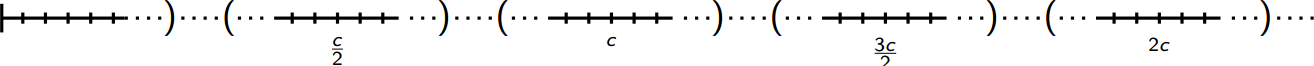
\includegraphics[scale=0.3]{nonstandard-model-of-arithmetic-cropped}
  \end{itemize}
\end{frame}

\backupend

\end{document}
